\chapter{INTRODUCTION}
\label{INTRODUCTION}
%\section*{Check}%
%\label{Check}
%The development of the Standard Model in the twentieth century is one of the greatest achievements of the particle physics which is a theory concerning the electromagnetic, weak, and strong nuclear interactions. The Standard Model states that the fundamental particles that make up all matter are quarks and leptons, and that they interact through the strong, weak, and electromagnetic fundamental interactions by exchanging force carrier particles. The Standard Model makes many predictions on nuclear and particle physics and many of them have been verified experimentally. Standard Model falls short of being a complete theory of fundamental interactions, one of them being parity violation.
%The Standard Model incorporates parity violation by expressing the weak interaction as a chiral gauge interaction.

The Q-weak experiment at the Thomas Jefferson National Accelerator Facility, USA, (TJNAF or JLab) is aimed to determine the weak charge of the proton by measuring parity-violating asymmetry of elastic electron-proton scattering at a low four-momentum-transfer squared ($Q^{2}$). The weak charge of the proton in the Standard Model (SM) is suppressed and any observed deviations from the SM predictions found in this high precision measurement will suggest signatures of new physics.


%%%%%%%%%%%%%%%%%%%%%%%%%%%%%%%%%%%%%%%%%%%%%%%%%%%%%%%%%%%%%%%%%%%%%%%
\section{The Standard Model and the Electroweak Interaction}
\label{The Standard Model and the Electroweak Interaction}

The development of the SM in the twentieth century is one of the greatest achievements of the particle physics which is a theory concerning the electromagnetic, weak, and strong nuclear interactions~\cite{book:QuarksAndLeptones}. 
%The SM states that the fundamental particles that make up all matter are quarks and leptons, and that they interact through the strong, weak, and electromagnetic fundamental interactions by exchanging force carrier particles. 
The SM states that quarks and leptons are the fundamental particles which comprise all matter, and they interact through strong, weak, and electromagnetic fundamental interactions by exchanging the force carrier particles.
A summary of the SM particles with their mass, charge, and spin is shown in Figure~\ref{fig:SMElementaryParticles}.
%The weak interaction is unique among the four known forces, because it is the only force known to violate parity. 
The weak interaction is unique among the four known forces since this is the only force known to violate the parity. 
A parity transformation is defined as a discrete change of spatial coordinates from ($x$,$y$,$z$) to ($-x$,$-y$,$-z$).
%A parity transformation is defined as a mirror reflection of a physical process, followed by a 180 degree rotation about the axis normal to the reflection plane. 
The electromagnetic and weak interactions have been unified in an electroweak theory, which is one of the several successes of the SM. The Prescott experiment~\cite{Prescott1978347} at the Stanford Linear Accelerator Center (SLAC) helped confirm the SM predictions of the weak neutral current for the first time~\cite{Hasert1973138, Hasert1973121, Hasert19741} by measuring the parity violating asymmetry in deep inelastic electron-deuteron scattering. 
Over the past half-a-century, the general structure of the SM was confirmed by many experiments.

%Experiments testing the SM can be categorized into three main branches: the energy frontier, the precision frontier, and the cosmological frontier. The high energy frontier experiments are designed to detect particles that are predicted by the SM or to detect new physics particles. The most prominent discovery machines include the Super Proton Synchrotron (SPS), the Large Electron Positron (LEP) collider also known as the Z factory, the Large Hadron Collider (LHC), and the Tevatron. They have discovered SM particles including the W and Z bosons [6] (at SPS), a Higgs like boson [7, 8] (at LHC), and the top quark [9, 10] (at Tevatron). The precision frontier experiments measure SM predicted quantities (ideally suppressed) to high precision or detect rare processes predicted by the SM. Therefore, precision frontier experiments are very diverse and vary from table-tops to colliders. Their results for SM predicted quantities can be used to constraint or develop new physics models beyond the SM. Examples of high precision measurements include the measurement of the anomalous magnetic moment of the electron or the muon [5, 11], the measurements of neutrino oscillations [12], the Electric Dipole Moment (EDM) measurements of leptons and nucleons [13], and the measurement of the weak charge of the proton by Qweak . Examples of attempted rare process detections include Majorana neutrino searches by using neutrinoless double β decays [14], dark matter searches [15], and matter anti-matter asymmetry studies performed at Large Hadron Collider beauty (LHCb) experiment [16]. The cosmological frontier experiments observe the visible and the dark universe using: cosmic ray studies [17], cosmic wave background measurements [18, 19], gravitational wave searches [20], dark matter searches [21], and matter anti-matter asymmetry direct and indirect measurements in space by Alpha Magnetic Spectrometer (AMS) experiment [22]. In summary, the energy frontier experiments are mainly discovery experiments where particles predicted by the SM or new particles can be discovered. The precision and cosmological frontier experiments mainly detect certain footprints or signatures that signal new physics and ultimately may lead to discoveries of new physics particles at the energy frontier. Therefore, all three branches of SM experiments are closely related. They test the SM and new physics theories essential to our understanding of the universe and a theory of everything. - Rakitha


\begin{singlespace}
\begin{figure}[h]
	\begin{center}
	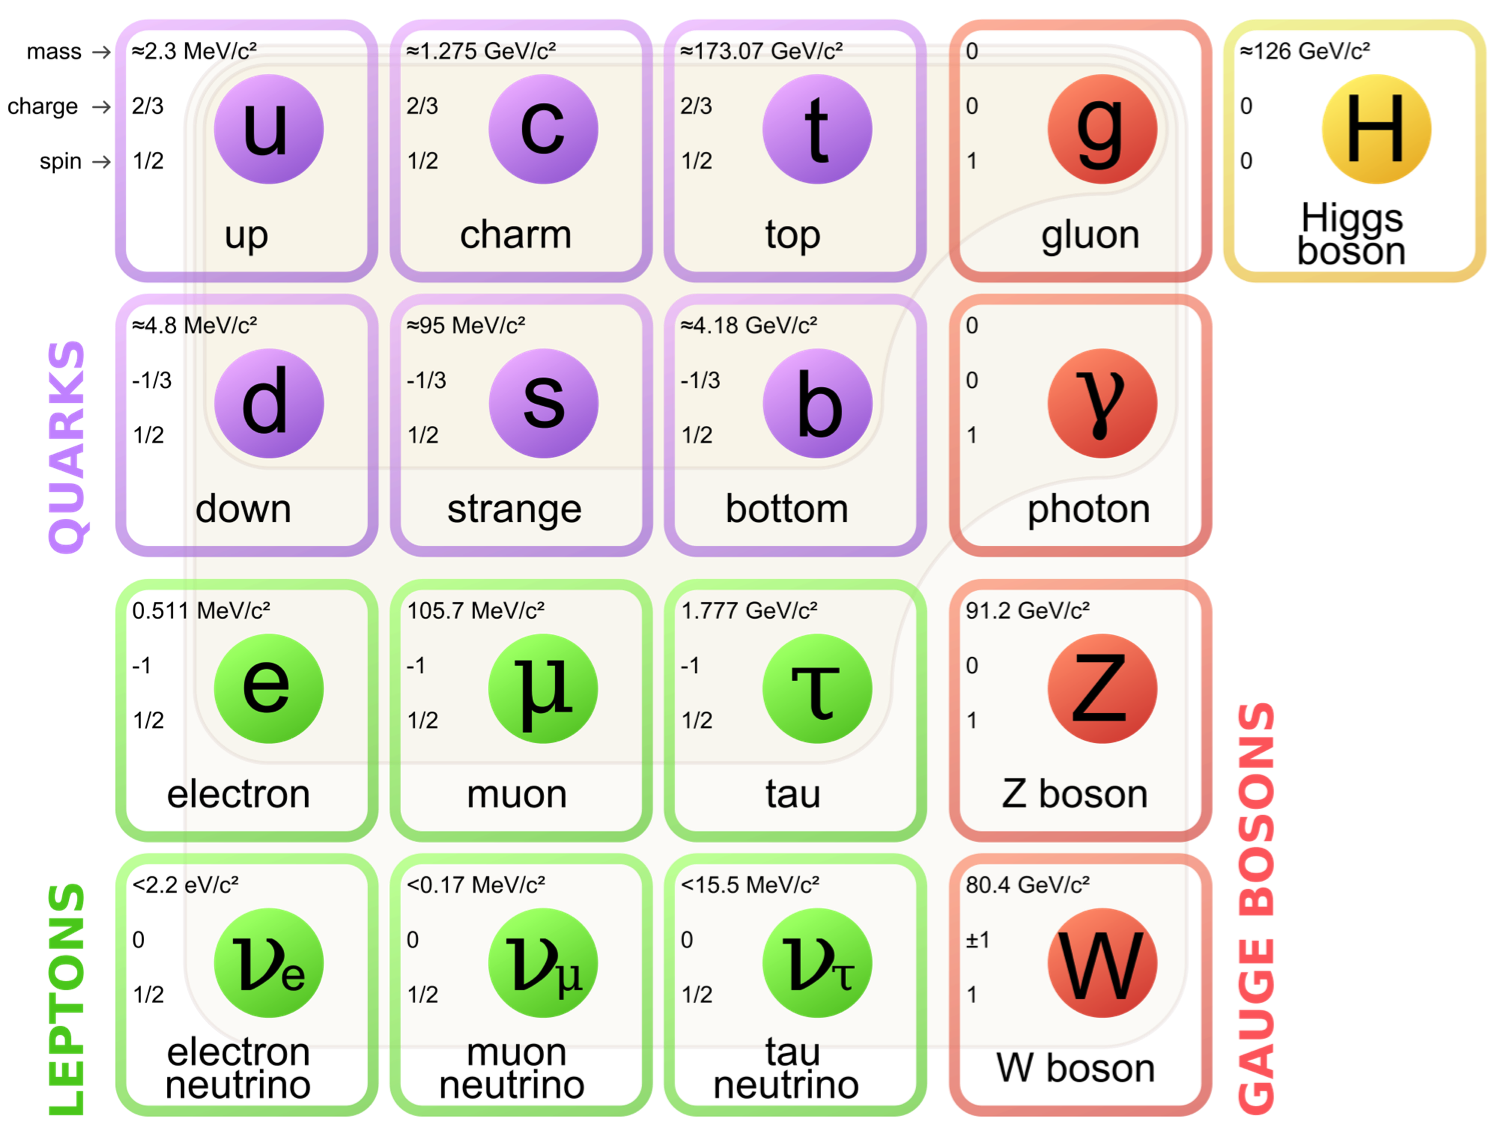
\includegraphics[width=15.0cm]{figures/SMElementaryParticles}
	\end{center}
	\caption
	[The Standard Model of elementary particles.]
	{The Standard Model of elementary particles~\cite{SM_figure}. The three generations of matter, gauge bosons are shown in the fourth column, whereas the newly discovered Higgs boson in the fifth.}
	\label{fig:SMElementaryParticles}
\end{figure}
\end{singlespace}

Despite many successes, there are many unresolved issues due to which the SM could not be claimed as a complete theory. One of such drawbacks is that the SM does not account for dark matter, dark energy, gravity, etc.
%Despite the many successes, there are also many reasons why the SM is not a complete theory. The  missing phenomena from the SM are dark matter, dark energy, gravity, etc. 
The recently observed 3$\sigma$ deviation of the anomalous magnetic moment of muon~\cite{PhysRevLett.92.161802} at Brookhaven National Laboratory could also be related to particle physics beyond the SM. 
%The SM falls short of being a complete theory of fundamental interactions, one of them being parity violation. 

The SM incorporates parity violation by expressing the weak interaction as a chiral gauge interaction. Over last the couple of decades, parity-violating electron scattering (PVES) has become an important experimental tool to investigate the contribution of the quark-antiquark sea of the nucleon to its electromagnetic structure. The advanced technologies and improved experimental techniques have allowed us to do challenging parity-violating experiments to measure parity-violating asymmetries at the parts-per-billion level.
Figure~\ref{fig:PVAsymmetry} shows a brief history of the measured asymmetry in different PVES experiments. The difficulty level of an experiment increases with the decrease of the size and precision of the asymmetry.  As shown in the Figure, the Q-weak experiment is expected to measure the most precise value of the PV asymmetry in e+p scattering to date. 

\begin{singlespace}
\begin{table}[!h]
\begin{center}
  	\caption
	[The electric and weak charges of elementary particles in the Standard Model.]
  	{The electric and weak charges of elementary particles in the Standard Model.}
  \begin{tabular}{ c | c | c  c  c }
%    \hline
    \noalign{\hrule height 1pt}
%    \multirow{2}{*}{Modulation asymmetry} & \multicolumn{3}{c}{Clock time required} \\
%    \cline{2-4}
     Particle & EM Charge & \multicolumn{3}{c}{Weak Charge} \\
%    \hline
    \noalign{\hrule height 1pt}
    u	& 2/3 & -2$C_{1u}$ & 1 - (8/3)$\sin^{2}\theta_{W}$ & $\sim$1/3 \\ 
    d	& 1/3 & -2$C_{1d}$ & 1 - (8/3)$\sin^{2}\theta_{W}$ & $\sim$1/3 \\ 
    p (uud)	& 1 & -2(2$C_{1u}+C_{1d}$) & 1 - 4$\sin^{2}\theta_{W}$ & $\sim$0.07 \\ 
    n (udd)	& 0 & -2(2$C_{1u}+C_{1d}$) & & $\sim$1 \\ 
%    \hline
    \noalign{\hrule height 1pt}
  	\end{tabular}
  \label{tab:SM_prediction}
\end{center}
\end{table}
\end{singlespace}


%%%%%%%%%%%%%%%%%%%%%%%%%%%%%%%%%%%%%%%%%%%%%%%%%%%%%%%%%%%%%%%%%%%%%%%
\section{The Q-weak Experiment}
\label{The Q-weak Experiment}

The SM makes a firm prediction of the weak charge of the proton ($Q^{p}_{W}$), based on the running of the weak mixing angle $\sin^{2}\theta_{W}$ from the $Z^{0}$ pole down to low energies. Any significant deviation of $\sin^{2}\theta_{W}$ from the SM prediction at low $Q^{2}$ would be a signal of new physics, whereas agreement would place new and significant constraints on possible SM extensions. 
The weak charge of the proton is suppressed in the SM (as shown in Table~\ref{tab:SM_prediction}), and a precise measurement will challenge the SM predictions and search for new physics. 

%The goal of the Q-weak experiment is to measure the parity violating asymmetry ($\sim$250~ppb) in elastic electron-proton scattering at $Q^{2}$ =0.03~(GeV/c)$^{2}$ and forward angles to determine the proton's weak charge with 4\% combined statistical and systematic uncertainties~\cite{qweak_proposal_2007}.
%In the absence of physics beyond the SM, the Q-weak experiment can provide a $\sim$0.3\% measurement of $\sin^{2}\theta_{W}$.
%A 2200~hours measurement using a 89\% polarized electron beam of 180~A on a 35~cm liquid Hydrogen target was performed during 2010 - 2012.

%A 2200~hours measurement of the PV asymmetry in elastic e+p scattering at $Q^{2}$ =0.03~(GeV/c)$^{2}$ employing 180~A of 89\% polarized beam on a 35~cm liquid Hydrogen target will determine the proton's weak charge with 4\% combined statistical and systematic errors. 
%
%A unique opportunity exists to carry out the first precision measurement of the proton's weak charge, $Q^{p}_{W}$ = 1 - 4$\sin^{2}\theta_{W}$, at JLab, building on technical advances that have been made in the laboratory's world-leading parity violation program and using the results of earlier experiments to constrain hadronic corrections. A 2200~hour measurement of the parity violating asymmetry in elastic e+p scattering at $Q^{2}$ =0.03~(GeV/c)$^{2}$ employing 180~A of 89\% polarized beam on a 35~cm liquid Hydrogen target will determine the proton's weak charge with 4\% combined statistical and systematic errors. 
%
%The Standard Model makes a firm prediction of $Q^{p}_{W}$, based on the running of the weak mixing angle $\sin^{2}\theta_{W}$ from the $Z^{0}$ pole down to low energies, corresponding to a 10 effect in our experiment. Any significant deviation of $\sin^{2}\theta_{W}$ from the Standard Model prediction at low Q2 would be a signal of new physics, whereas agreement would place new and significant constraints on possible Standard Model extensions. In the absence of physics beyond the Standard Model, our experiment will provide a 0.3\% measurement of $\sin^{2}\theta_{W}$, making this a very competitive stand alone measurement of the weak mixing angle.

\begin{singlespace}
\begin{figure}[h]
	\begin{center}
	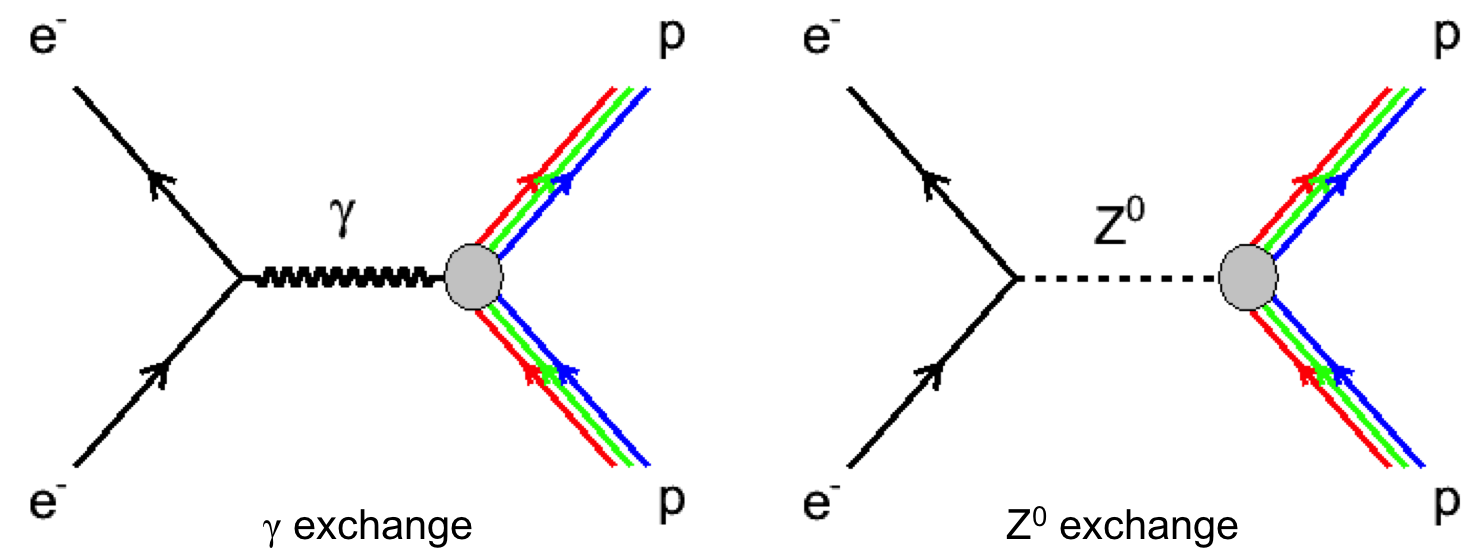
\includegraphics[width=15.0cm]{figures/FeynmanDiagramsPVES}
	\end{center}
	\caption
	[The Feynman diagrams for the parity conserving and parity violating semileptonic electroweak interactions.]
	{The Feynman diagrams for the parity conserving and parity violating semileptonic electroweak interactions.}
	\label{fig:FeynmanDiagramsPVES}
\end{figure}
\end{singlespace}


Neutral current electron-proton scattering can involve either an exchange of a photon or a $Z^{0}$ boson (Figure~\ref{fig:FeynmanDiagramsPVES}). The scattering cross section is a summation and an interference of the two invariant amplitudes.

\begin{equation} \label{equ:qweak1}
\sigma \approx \vert \mathcal{M}_{EM} + \mathcal{M}_{weak} \vert^{2} \approx \vert \mathcal{M}_{EM} \vert^{2} + 2 \Re \mathcal{M}_{EM}^{*}\mathcal{M}_{weak} + \vert \mathcal{M}_{weak} \vert^{2}, 
\end{equation}

Here $\mathcal{M}_{EM}$, and $\mathcal{M}_{weak}$ are the amplitudes for the exchange of a photon and $Z^{0}$ boson, respectively. 
The sign of $\mathcal{M}_{weak}$ changes the sign of the interference term under a parity transformation. Experimentally, this is achieved by changing the helicity of a longitudinally polarized electron scattering from an unpolarized nucleon. The parity-violating asymmetry is then defined as

%\begin{equation} \label{equ:qweak2}
%A_{PV} = \frac{\overset{{}_{\rightarrow}}{\sigma} - \overset{{}_{\leftarrow}}{\sigma} }{\overset{{}_{\rightarrow}}{\sigma} + \overset{{}_{\leftarrow}}{\sigma}},
%\end{equation}
\begin{equation} \label{equ:qweak2}
A_{PV} = \frac{\sigma^{+} - \sigma^{-} }{\sigma^{+} + \sigma^{-}},
\end{equation}

\noindent
%where $\overset{{}_{\rightarrow}}{\sigma}$($\overset{{}_{\leftarrow}}{\sigma}$) 
where $\sigma^{+}$ ($\sigma^{-}$)
is the cross section for the electrons scattering with spin polarized parallel (anti-parallel) to their direction of motion.
Given that $\vert \mathcal{M}_{weak} \vert \ll \vert \mathcal{M}_{EM} \vert$, this asymmetry reduces to being proportional to

\begin{equation} \label{equ:qweak3}
A_{PV} \sim \frac{2 \mathcal{M}_{weak} \mathcal{M}_{EM}}{\vert \mathcal{M}_{EM} \vert^{2}}.
\end{equation}

At tree level, the full form of the asymmetry for electron-proton scattering can be written as~\cite{qweak_proposal_2007}

\begin{equation} \label{equ:qweak4}
A_{PV} = \left[ \frac{-G_{F}Q^{2}}{4 \sqrt{2}\pi\alpha} \right] \left[ \frac{{\varepsilon} {G_{E}^{p\gamma}}G_{E}^{pZ} + {\tau} {G_{M}^{p\gamma}}G_{M}^{pZ} - (1-4\sin^{2}\theta_{W}){\varepsilon^{\prime}}{G_{M}^{p\gamma}}{G_{A}^{e}} } { {\varepsilon}({G_{E}^{p\gamma}})^{2} + {\tau}({G_{M}^{p\gamma}})^{2} } \right],
\end{equation}

\noindent
where the Fermi constant is denoted by $G_{F}$. The kinematic factors in terms of proton mass $M$, scattering angle $\theta$, and four-momentum transfer squared $Q^{2}$ are given by

\begin{equation} \label{equ:qweak5}
{\varepsilon} = \frac{1}{1 + 2(1+{\tau})\tan^{2}\frac{\theta}{2}}, {\varepsilon^{\prime}} = \sqrt{{\tau}(1+{\tau})(1 - {\varepsilon}^{2})}, {\tau} = \frac{Q^{2}}{4M},
\end{equation}

\noindent
and electromagnetic form factors can be expressed as

\begin{equation} \label{equ:qweak6}
G_{E,M}^{pZ} = (1 - 4\sin^{2} \theta_{W}) {G_{E,M}^{p\gamma}} - {G_{E,M}^{n\gamma}} - {G_{E,M}^{s}}.
\end{equation}

The weak charge of the proton in the SM is given by 

\begin{equation} \label{equ:qweak7}
Q_{W}^{p} = (1-4\sin^{2}\theta_{W}).
\end{equation}

\noindent
Defining 

\begin{equation} \label{equ:qweak8}
A_{0} = \frac{-G_{F}Q^{2}}{4 \sqrt{2}\pi\alpha},
\end{equation}

\noindent
and using equations~\ref{equ:qweak4}, \ref{equ:qweak5}, \ref{equ:qweak6}, \ref{equ:qweak7}, the reduced asymmetry can be written as 

\begin{equation} \label{equ:qweak9}
\frac{A_{PV}}{A_{0}} = \left[ \frac{{\varepsilon} {G_{E}^{p\gamma}} (Q_{W}^{p} {G_{E}^{p\gamma}} - {G_{E}^{n\gamma}} - {G_{E}^{s}} ) + {\tau} {G_{M}^{p\gamma}} (Q_{W}^{p} {G_{M}^{p\gamma}} - {G_{M}^{n\gamma}} - {G_{M}^{s}} ) - (1-4\sin^{2}\theta_{W}){\varepsilon^{\prime}}{G_{M}^{p\gamma}}{G_{A}^{e}} } { {\varepsilon}({G_{E}^{p\gamma}})^{2} + {\tau}({G_{M}^{p\gamma}})^{2} } \right]
\end{equation}

%\begin{dmath}\label{equ:qweak5}
%
%\end{dmath}

%\begin{equation} \label{equ:qweak10}
%\frac{A_{PV}}{A_{0}} = Q_{W}^{p}\left[ \frac{{\varepsilon}({G_{E}^{p\gamma}})^{2} + {\tau}({G_{M}^{p\gamma}})^{2} }{ {\varepsilon}({G_{E}^{p\gamma}})^{2} + {\tau}({G_{M}^{p\gamma}})^{2} } \right] + \left[(-1)\frac{{\varepsilon}{G_{E}^{p\gamma}}{G_{E}^{n\gamma}} + {\tau}{G_{M}^{p\gamma}}{G_{M}^{n\gamma}} }{ {\varepsilon}({G_{E}^{p\gamma}})^{2} + {\tau}({G_{M}^{p\gamma}})^{2} } \right]  + \left[(-1)\frac{(1-4\sin^{2}\theta_{W}){\varepsilon^{\prime}}{G_{M}^{p\gamma}}{G_{A}^{e}} }{ {\varepsilon}({G_{E}^{p\gamma}})^{2} + {\tau}({G_{M}^{p\gamma}})^{2} } \right].
%\end{equation}
\begin{equation} \label{equ:qweak10}
\frac{A_{PV}}{A_{0}} = Q_{W}^{p} + \left[(-1)\frac{{\varepsilon}{G_{E}^{p\gamma}}{G_{E}^{n\gamma}} + {\tau}{G_{M}^{p\gamma}}{G_{M}^{n\gamma}} }{ {\varepsilon}({G_{E}^{p\gamma}})^{2} + {\tau}({G_{M}^{p\gamma}})^{2} } \right]  + \left[(-1)\frac{(1-4\sin^{2}\theta_{W}){\varepsilon^{\prime}}{G_{M}^{p\gamma}}{G_{A}^{e}} }{ {\varepsilon}({G_{E}^{p\gamma}})^{2} + {\tau}({G_{M}^{p\gamma}})^{2} } \right].
\end{equation}

%\begin{equation} \label{equ:qweak5}
%A_{Q-weak} = \left[ \frac{-G_{F}Q^{2}}{4 \sqrt{2}\pi\alpha} \right] Q_{W}^{p}\left[ \frac{{\varepsilon}({G_{E}^{p\gamma}})^{2} + {\tau}({G_{M}^{p\gamma}})^{2} }{ {\varepsilon}({G_{E}^{p\gamma}})^{2} + {\tau}({G_{M}^{p\gamma}})^{2} } \right] 
%\end{equation}

%\begin{equation} \label{equ:qweak5}
%A_{Q-weak} = \left[ \frac{-G_{F}Q^{2}}{4 \sqrt{2}\pi\alpha} \right] Q_{W}^{p}
%\end{equation}
%
%\begin{equation} \label{equ:qweak5}
%A_{hadronic} = \left[ \frac{-G_{F}Q^{2}}{4 \sqrt{2}\pi\alpha} \right] Q_{W}^{n}\left[\frac{{\varepsilon}{G_{E}^{p\gamma}}{G_{E}^{n\gamma}} + {\tau}{G_{M}^{p\gamma}}{G_{M}^{n\gamma}} }{ {\varepsilon}({G_{E}^{p\gamma}})^{2} + {\tau}({G_{M}^{p\gamma}})^{2} } \right] 
%\end{equation}
%
%\begin{equation} \label{equ:qweak5}
%A_{axial} = \left[ \frac{-G_{F}Q^{2}}{4 \sqrt{2}\pi\alpha} \right] G_{A}^{e}\left[\frac{(1-4\sin^{2}\theta_{W}){\varepsilon^{\prime}}{G_{M}^{p\gamma}}{G_{A}^{Z}} }{ {\varepsilon}({G_{E}^{p\gamma}})^{2} + {\tau}({G_{M}^{p\gamma}})^{2} } \right] 
%\end{equation}

The total reduced asymmetry can be expressed as a combination of three reduced asymmetries as following

\begin{equation} \label{equ:qweak11}
\frac{A_{PV}}{A_{0}} = A_{Q-weak}  + A_{hadronic}  + A_{axial}.
\end{equation}


Here individual asymmetries are

\begin{equation} \label{equ:qweak12}
A_{Q-weak} = Q_{W}^{p},
\end{equation}

\begin{equation} \label{equ:qweak13}
A_{hadronic} = Q_{W}^{n}\left[\frac{{\varepsilon}{G_{E}^{p\gamma}}{G_{E}^{n\gamma}} + {\tau}{G_{M}^{p\gamma}}{G_{M}^{n\gamma}} }{ {\varepsilon}({G_{E}^{p\gamma}})^{2} + {\tau}({G_{M}^{p\gamma}})^{2} } \right],
\end{equation}

\begin{equation} \label{equ:qweak14}
A_{axial} = - G_{A}^{e}\left[\frac{(1-4\sin^{2}\theta_{W}){\varepsilon^{\prime}}G_{M}^{p\gamma} }{ {\varepsilon}({G_{E}^{p\gamma}})^{2} + {\tau}({G_{M}^{p\gamma}})^{2} } \right],
\end{equation}

\noindent
where the contribution from the strange form factors is ignored.

Under the kinematic condition of $\theta$ $\rightarrow$ 0, $\varepsilon$ $\rightarrow$ 1, and $\tau$ $\ll$ 1, the asymmetry simplifies as 

\begin{equation} \label{equ:qweak15}
\frac{A_{PV}}{A_{0}} = Q_{W}^{p} + Q^{2}B(Q^{2}, \theta),
\end{equation}

\noindent
where the B($Q^{2}$,$\theta$) term contains the hadronic contribution to the asymmetry and is about 30\%. Previous PVES experiments at higher $Q^{2}$ constrain this latter contribution.

%\begin{equation} \label{equ:qweak51}
%\frac{A_{ep}}{A_{0}} = \left[ Q_{W}^{p} + Q^{2} B(Q^{2}, \theta) \right]
%\end{equation}

%\begin{equation} \label{equ:qweak3}
%A_{ep} = \left[ \frac{-G_{F}Q^{2}}{4 \sqrt{2}\pi\alpha} \right] \left[ Q_{W}^{p} + B(Q^{2}, \theta) \right] = A_{0} \left[ Q_{W}^{p} + B(Q^{2}, \theta) \right]
%\end{equation}

%\begin{equation} \label{equ:qweak5}
%A_{ep} = \left[ \frac{-G_{F}Q^{2}}{4 \sqrt{2}\pi\alpha} \right] \left[ Q_{W}^{p} + Q^{2}B(Q^{2}, \theta) \right] = A_{0} \left[ Q_{W}^{p} + Q^{2}B(Q^{2}, \theta) \right]
%\end{equation}

%
%\begin{equation} \label{equ:qweak4}
%\begin{split}
%A_{ep} = A_{0} \left[ Q_{W}^{p} + B(Q^{2}, \theta) \right]\\
%A_{0} = \frac{-G_{F}Q^{2}}{4 \sqrt{2}\pi\alpha}
%\end{split}
%\end{equation}


%\begin{equation} \label{equ:qweak6}
%\begin{split}
%\sigma \approx \vert M_{EM} + M_{weak} \vert^{2} \\
%\sigma \approx \vert M_{EM} \vert^{2} + 2M_{EM}^{*}M_{weak} + \vert M_{weak} \vert^{2}  \\
%\sigma \approx \vert M_{EM} \vert^{2} 
%\end{split}
%\end{equation}
%

\begin{singlespace}
\begin{figure}[!h]
	\begin{center}
	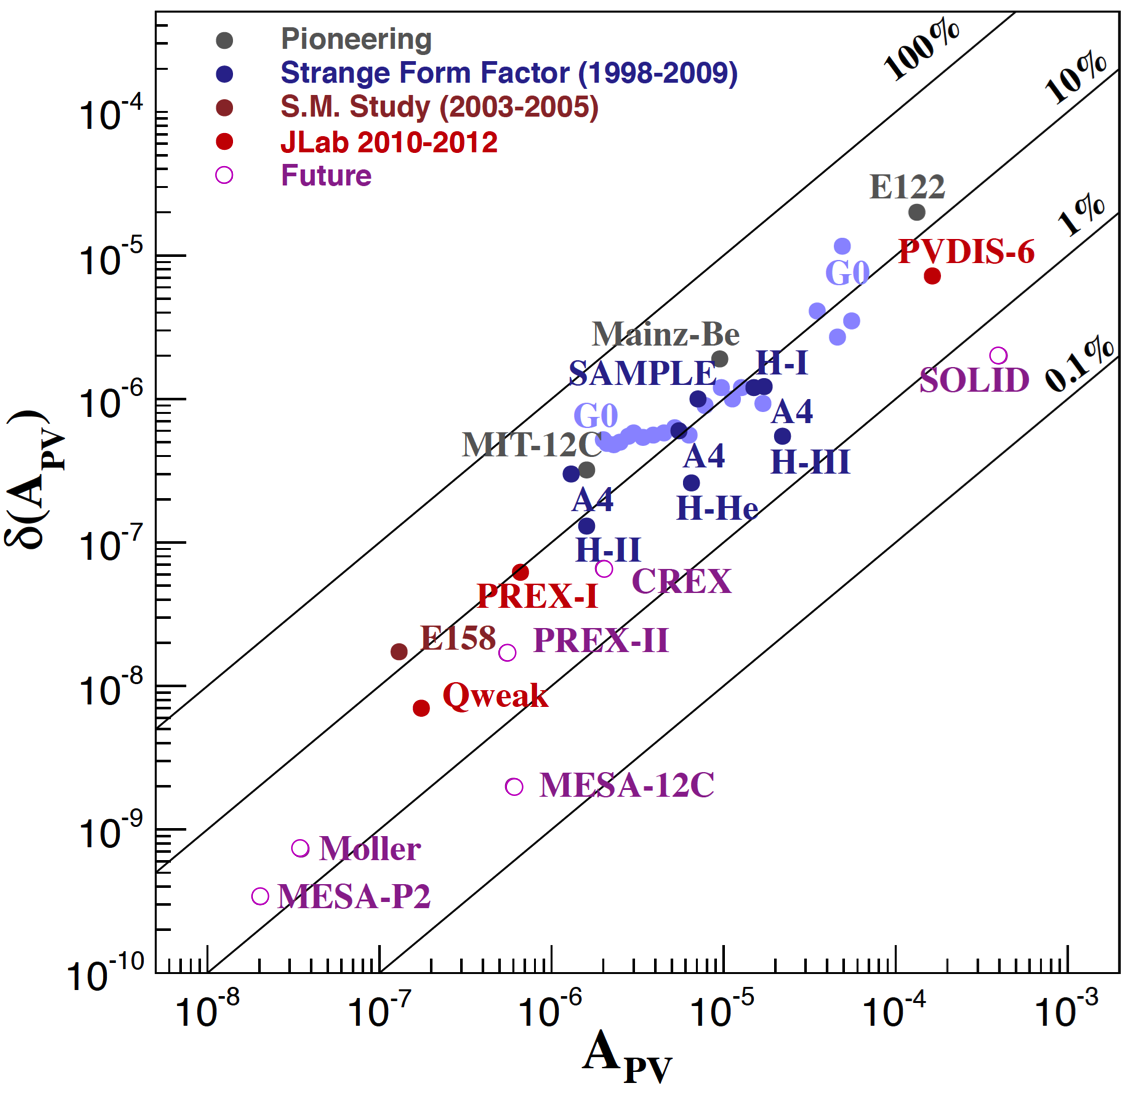
\includegraphics[width=15.0cm]{figures/PVAsymmetry}
	\end{center}
	\caption
	[Q-weak will be most precise (relative and absolute) PVES result to date.]
	{Q-weak will be most precise (relative and absolute) PVES result to date.}
	\label{fig:PVAsymmetry}
\end{figure}
\end{singlespace}

The goal of the Q-weak experiment is aimed to measure this parity violating asymmetry ($\sim$250~ppb) in elastic electron-proton scattering at $Q^{2}$ = 0.025~(GeV/c)$^{2}$ and forward angles to determine the proton's weak charge with 4\% combined statistical and systematic uncertainties~\cite{qweak_proposal_2007}.
The experiment will also provide a $\sim$0.3\% measurement of the weak mixing angle. 
A 2200~hours measurement using a 88\% polarized electron beam of 180~$\mu$A on a 35~cm liquid Hydrogen target was performed during 2010 - 2012.


%%%%%%%%%%%%%%%%%%%%%%%%%%%%%%%%%%%%%%%%%%%%%%%%%%%%%%%%%%%%%%%%%%%%%%%
\section{Inelastic Parity Violating Asymmetry}
\label{Inelastic Parity Violating Asymmetry}

In addition to measuring the elastic PV asymmetry for Q-weak, dedicated data were taken to extract the inelastic PV asymmetry in electron-proton scattering. During normal production running, the detector signals were integrated to obtain the yield and the inelastic events reach into the detector acceptance. There is no clear way to separate the inelastic signal from the elastic signal. The inelastic asymmetry is expected to be a factor of 10 larger than the elastic asymmetry, and hence, it was critical to measure the inelastic dilution and correct for it. The inelastic contribution in the Q-weak acceptance is mainly dominated by the production of the resonance.

%In addition to measuring the elastic asymmetry for Q-weak, dedicated time is allotted to
%measure the inelastic asymmetry. Inelastic events make it into the acceptance during normal
%production running and, because we integrate the detector signals, there is no way to separate
%the inelastic signal from the elastic signal. The inelastic asymmetry is expected to be a factor
%of 10 larger than the elastic asymmetry so knowing how many inelastic events are present is
%critical for correcting for the inelastic contribution.
%The inelastic contribution in the Q-weak acceptance is dominated by the production of the resonance. The Feynman diagram for the inelastic interaction for Q-weak is given in Figure 2.5. The incident electron (e) interacts with the proton (p) and loses energy (e'). The lost energy is transferred to the proton, which is excited to its first resonance (+) then decays to a neutral pion ($\pi^{0}$) and a proton (p). - Leacock

%%-------------------------------------------------------------------%%
\subsection{The $\Delta$ Resonance}
\label{The Delta Resonance}

The $\Delta$ is the first resonance of the nucleon with nucleon spin $J$=3/2 and mass 1232~MeV. In the ground state, the total spin of the proton is $J$=1/2 and is the sum of the spins of its constituent quarks (uud). The nucleon has two valance quark spins aligned parallel and one antiparallel. Therefore, only two possible flavor states (uud, udd) exist corresponding to isospin 1/2, whereas the $\Delta$ baryons have all three quark spins aligned parallel~\cite{Klempt:2002cu}. A list of allowed $\Delta$ resonance states and their properties is given in Table~\ref{tab:delta_resonance}.

%The Delta baryons are a spin excitation of the nucleon doublet. Since the nucleon is the non-strange isospin-1/2 group in the JP = 1/2+ octet (ground state), the Delta resonances are the spin-excited equivalent in the JP = 3/2- decuplet. While the nucleon will have two quark spins aligned and one opposite, and hence only two possible flavor states (uud, udd) corresponding to isospin-1/2, the Delta baryons will have all three quark spins aligned. This allows for the isospin to extend to 3/2 for the Delta's, so there are four possible flavor states (uuu, uud, udd, ddd). The bag model gives a good estimate for the masses of the Delta's in relation to the nucleons, and so does the basic vector-gluon exchange model, both with simple expressions.

\begin{singlespace}
\begin{table}[!h]
\begin{center}
  	\caption
	[Nucleons and $\Delta$ resonances and their associated properties.]
  	{Nucleons and $\Delta$ resonances and their associated properties.}
  \begin{tabular}{ l | c  c  c  c  c }
%    \hline
    \noalign{\hrule height 1pt}
%    \multirow{2}{*}{Modulation asymmetry} & \multicolumn{3}{c}{Clock time required} \\
%    \cline{2-4}
     Particle	& Quarks		& EM Charge	& Spin	& Isopin		& $I_{3}$ \\
%    \hline
    \noalign{\hrule height 1pt}
    p				& uud	& +1		& $\uparrow\uparrow\downarrow$	& 1/2	& +1/2 \\ 
    n				& udd	& 0		& $\uparrow\downarrow\downarrow$	& 1/2	& -1/2 \\ 
    $\Delta^{++}$	& uuu	& +2		& $\uparrow\uparrow\uparrow$		& 3/2	& +3/2 \\ 
    $\Delta^{+}$		& uud	& +1		& $\uparrow\uparrow\uparrow$		& 3/2	& +1/2 \\ 
    $\Delta^{0}$		& udd	& 0		& $\uparrow\uparrow\uparrow$		& 3/2	& -1/2 \\ 
    $\Delta^{-}$		& ddd	& -1		& $\uparrow\uparrow\uparrow$		& 3/2	& -3/2 \\ 
%    \hline
    \noalign{\hrule height 1pt}
  	\end{tabular}
  \label{tab:delta_resonance}
\end{center}
\end{table}
\end{singlespace}

A photon or Z boson can interact with a nucleon and flip the spin of one of the quarks to make them all parallel to produce a $\Delta$ baryon. 
Only a $\Delta^{+}$ or $\Delta^{0}$ can be created by this kind of interaction if the target particle is a proton or neutron, respectively. On the other hand, weakly interacting particle, such as a neutrino, a quark can change flavor and flip the spin to produce $\Delta^{++}$ and $\Delta^{-}$. 
An electron-proton interaction induces a quark spin flip and can reveal information about how the quark spin is redistributed during the transition. For the Q-weak experiment where the interactions were predominantly electron-proton, only the relevant resonance $\Delta^{+}$ is considered.

%A  can be created in a number of ways. A photon could interact with a nucleon and 
%ip
%the spin of one of the quarks to make them all parallel. A Z boson can create a  in the
%same way. These reactions can only create a + or a 0 if the target particle is a proton or
%neutron, respectively. However, if a nucleon is struck by a charged current weakly interacting
%particle, such as a neutrino, a quark can change 
%avor (from up to down or down to up) and
%
%ip spin. This reaction can create the ++ and the 􀀀. For the purposes of this thesis and
%Qweak, only the + is considered. A plot showing the rst few resonances of the proton is
%shown in Figure 2.1. The relatively broad peak at 1.2 GeV is the  resonance discussed
%in this thesis. The width is related to the lifetime of the resonance by Equation 2.1. The
%dominant decay mode for all  states is via the strong force into a nucleon and a pion.
%
%The width of the  resonance is 118 MeV. Using Equation 2.1 one nds the lifetime of the
% to be 5.5810􀀀24 s. Relatively short lifetimes are due to decays via the strong force. If a
%particle can only decay via the weak force the lifetime is longer, e.g. the muon has a lifetime
%of 2.210􀀀6 s and the free neutron has a lifetime of 880 s [6].
%
%An electron-proton interaction that induces a quark spin 
%ip will reveal information about
%how the quark spin is redistributed during the transition. This information is contained in
%the axial transition form factor, GA
%N.

\begin{singlespace}
\begin{figure}[h]
	\begin{center}
	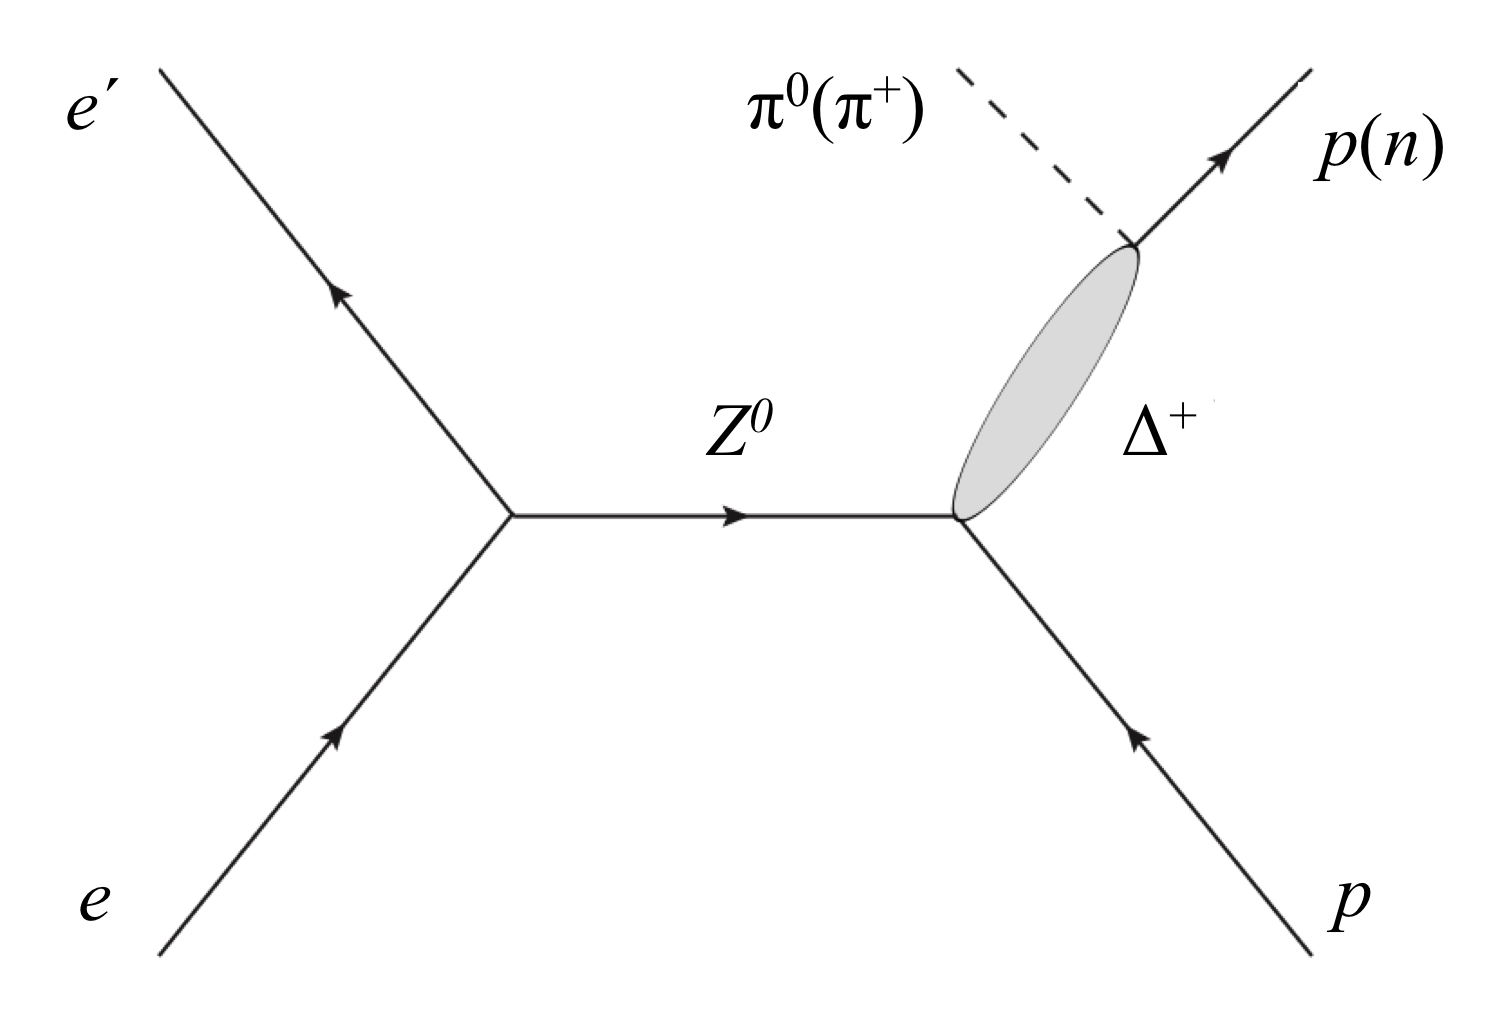
\includegraphics[width=8.0cm]{figures/FeynmanDiagramsPVN2Delta}
	\end{center}
	\caption
	[The Feynman diagrams for the parity violating inelastic electron-proton scattering.]
	{The Feynman diagrams for the parity violating inelastic electron-proton scattering~\cite{leacock_qweak}.}
	\label{fig:FeynmanDiagramsPVN2Delta}
\end{figure}
\end{singlespace}


%%-------------------------------------------------------------------%%
\subsection{Formalism and Measurement}%
\label{Formalism and Measurement}

In inelastic PV electron-proton scattering, the incident electron interacts with the proton and loses energy. The proton absorbs this energy and get excited to its first resonance ($\Delta^{+}$), then decays to a neutral pion ($\pi^{0}$) and a proton (as shown in Figure~\ref{fig:FeynmanDiagramsPVN2Delta}).
The parity-violating asymmetry in the nucleon $\rightarrow$ $\Delta$ transition can be expressed as~\cite{Mukhopadhyay1998481,PhysRevD.65.033001}

\begin{equation} \label{equ:qweak16}
A_{PV}^{in} = \left[ \frac{-G_{F}Q^{2}}{4 \sqrt{2}\pi\alpha} \right] \left[ \Delta_{(1)}^{\pi} + \Delta_{(2)}^{\pi} + \Delta_{(3)}^{\pi} \right],
\end{equation}

\noindent
where $\Delta_{(1)}^{\pi}$ contains the resonant terms, which are all isovector, $\Delta_{(2)}^{\pi}$ contains the nonresonant terms including both isovector and isoscalar, and $\Delta_{(3)}^{\pi}$ contains all axial-vector reactions at the hadron vertex.
The contribution of the inelastic PV to the Q-weak asymmetry is small.
%The torodial magnet current was reduced to focus inelastically scattered electrons onto the main \v{C}erenkov detectors. 
%As part of a program of inelastic PV asymmetry background studies, we made the first measurement of beam normal single spin asymmetry in the nucleon $\rightarrow \Delta$ transition using the Q-weak apparatus.
The asymmetry for the N $\rightarrow \Delta$ transition was measured as a part of the Q-weak background studies. 
%As part of a Q-weak asymmetry background studies, we made the  measurement of beam normal single spin asymmetry in the nucleon $\rightarrow \Delta$ transition using the Q-weak apparatus.


%%%%%%%%%%%%%%%%%%%%%%%%%%%%%%%%%%%%%%%%%%%%%%%%%%%%%%%%%%%%%%%%%%%%%%%
\section{The Beam Normal Single Spin Asymmetry}%
\label{The Beam Normal Single Spin Asymmetry}

The beam normal single spin asymmetry (BNSSA) is generated by polarized electrons when scattered from unpolarized protons and is a possible false background asymmetry in parity violating electron scattering experiments (PVES). 
The BNSSA is a  parity conserving asymmetry. Theoretical calculations~\cite{Arrington2011782} indicates that, the size of this asymmetry can be several orders of magnitude larger than that of the parity violating asymmetry.
For a precision experiment like Q-weak, it was important to estimate the background due to BNSSA and a dedicated measurement was performed. 
%Besides BNSSA provides direct access to the two-photon exchange process which is required to properly estimate the electron-nucleon scattering cross-sections beyond the Born approximation.

%The beam normal single spin asymmetry (BNSSA) generated by the scattering of polarized electrons from unpolarized protons is a possible false background asymmetry in parity violating electron scattering experiments (PVES). Theoretical calculations of the size of this parity conserving asymmetry indicates that it can be several orders of magnitude larger than the parity violating asymmetry. This prompted the Q-weak collaboration to make a dedicated measurement of the beam normal single spin asymmetry. But in its own perspective, a beam normal single spin asymmetry measurement provides direct access to the two-photon exchange process which is required to properly estimate the electron-nucleon scattering cross-sections beyond the Born approximation as discussed in the following subsections. - Buddhini


Elastic electron-nucleon scattering in the one-photon exchange approximation gives a direct access to the electromagnetic form factors of the nucleon which contains information about its structure. The ratio of the proton's electric to magnetic form factors ($G_{Ep}$/$G_{Mp}$) has been measured precisely up to large momentum transfer ($Q^{2}$) in the precision experiments using two different methods, namely the polarization transfer~\cite{PhysRevLett.84.1398, PhysRevLett.88.092301} and unpolarized measurements~\cite{PhysRevD.50.5491, PhysRevC.70.015206, Arrington:2003tq} using the Rosenbluth separation technique. These two different methods shows inconsistent results.
This puzzle may be explained by a two-photon exchange amplitude whose magnitude is a few percent of the one
photon exchange term as shown in~\cite{PhysRevLett.91.142303}.
A beam normal single spin asymmetry measurement provides a direct access to the two-photon exchange process which is required to properly estimate the electron-nucleon scattering cross-sections beyond the Born approximation.


%%%%%%%%%%%%%%%%%%%%%%%%%%%%%%%%%%%%%%%%%%%%%%%%%%%%%%%%%%%%%%%%%%%%%%%
\section{Inelastic Beam Normal Single Spin Asymmetry}%
\label{Inelastic Beam Normal Single Spin Asymmetry}

%Elastic electron–nucleon scattering in the one-photon exchange approximation gives
%direct access to the electromagnetic form factors of the nucleon, an essential piece of
%information about its structure. - Gorchtein

There is a parity conserving BNSSA or transverse asymmetry ($B_{n}$) on H$_{2}$ with a $\sin(\phi)$-like dependence due to two-photon exchange. The size of $B_{n}$ is few ppm, so a few percent residual transverse polarization in the beam, in addition to potentially small broken azimuthal asymmetries in the main detector, might lead to few ppb corrections to the Q-weak data. As part of a program of $B_{n}$ background studies, the first measurement of $B_{n}$ in the N$\rightarrow\Delta$ transition was performed using the Q-weak apparatus. 
%$B_{n}$ from electron-nucleon scattering is also a unique tool to study the $\gamma^{*}\Delta\Delta$ form factors~\cite{Alexandrou:2009hs}. 
%This chapter contains the details of the analysis on transverse asymmetry in  N-to-$\Delta$ region for H$_{2}$ target.


%%%%%%%%%%%%%%%%%%%%%%%%%%%%%%%%%%%%%%%%%%%%%%%%%%%%%%%%%%%%%%%%%%%%%%%
\section{Thesis Outline}%
\label{Thesis Outline}

%This dissertation will present a preliminary analysis of the beam normal single spin asymmetry measured from inelastic electron-proton scattering using the Q-weak apparatus. This chapter gives a motivation for the Q-weak experiment and provides an brief overview of the theory of beam normal single spin asymmetry measurements, while chapter~\ref{EXPERIMENTAL SETUP} gives a description of the experimental apparatus, and chapter~\ref{BEAM MODULATION} provides a detailed description of the beam modulation system. Application of beam modulation system, beamline characterization, and pedestal survey are summarized in chapter~\ref{BEAMLINE OPTICS AND FALSE ASYMMETRIES}. Chapter~\ref{BEAM NORMAL SINGLE SPIN ASYMMETRY} gives details of the data analysis and treatment of systematic uncertainties of beam normal single spin asymmetry in inelastic e+p scattering. The final result is summarized and discussed in chapter~\ref{CONCLUSIONS}.

This dissertation will present a preliminary analysis of the beam normal single spin asymmetry measured from the inelastic electron-proton scattering using the Q-weak apparatus. The outline of this dissertation is organized as follows:

\begin{itemize}
\doublespacing
%\item chapter~\ref{INTRODUCTION}: a motivation for the Q-weak experiment and an brief overview of the theory of beam normal single spin asymmetry measurements,
\item chapter~\ref{INTRODUCTION}: INTRODUCTION - an introduction and motivation for the Q-weak experiment,
\item chapter~\ref{THEORY}: THEORY - an brief overview of the theory of beam normal single spin asymmetry measurements,
\item chapter~\ref{EXPERIMENTAL SETUP}: EXPERIMENTAL SETUP - a brief description of the experimental apparatus,
\item chapter~\ref{BEAM MODULATION}: BEAM MODULATION - provides a detailed description of the beam modulation system,
\item chapter~\ref{BEAMLINE OPTICS AND FALSE ASYMMETRIES}: BEAMLINE OPTICS AND FALSE ASYMMETRIES - application of beam modulation system, beamline characterization, and pedestal survey,
\item chapter~\ref{BEAM NORMAL SINGLE SPIN ASYMMETRY}: BEAM NORMAL SINGLE SPIN ASYMMETRY - gives details of the data analysis and treatment of systematic uncertainties of beam normal single spin asymmetry in inelastic e+p scattering,
\item chapter~\ref{DISCUSSION AND CONCLUSIONS}: DISCUSSION AND CONCLUSIONS - a summary of the emphasized work and analysis status.
%the final result is summarized and discussed.
\end{itemize}



%\renewcommand{\arraystretch}{1.0} % make cell wider
%\begin{table}[!h]
% \begin{center}
%   \caption
%	[Transverse N-to-$\Delta$ data set.]   
%   {Transverse N-to-$\Delta$ data set. The data set for vertical transverse polarization are in parenthesis, rest are from horizontal transverse polarization. The beam current for different targets are shown in second last row. Amount of transverse data collected in terms of the total charge in Coulombs are shown in bottom row.}
%  \begin{tabular}{ c | c | c  c  c | c  c }
%%    \hline
%    \noalign{\hrule height 1pt}
%%    \multirow{2}{*}{HWP} & QTor current  & & QTor current & &  \multicolumn{2}{c}{QTor current} \\
%    \multirow{3}{*}{IHWP} & \multicolumn{6}{c}{QTor current} \\ \cline{2-7}
%%	\cline{2-7}%\hline
%		 &  6000 A & & 6700 A & &  \multicolumn{2}{c}{7300 A}\\
%	\cline{2-7}%\hline
%	     & LH$_{2}$ & LH$^{\dagger}_{2}$ & Al$^{\dagger\dagger}$ & $^{12}$C &  LH$_{2}$ & Al \\
%%	\cline{2-7}%\hline
%    \noalign{\hrule height 1pt}
%%    \hline
%	IN  & \pbox{3cm}{16152\\ 16153} & \pbox{3cm}{(16066)\\ 16131\\ 16132} & \pbox{3cm}{(16067)\\ 16115\\ 16116} & \pbox{3cm}{16150\\ 16151} & \pbox{3cm}{16133\\ 16134\\ 16135} & \pbox[c][2cm][c]{3cm}{ 16122\\ 16123\\ 16124\\ 16160 } \\ 
%    \noalign{\hrule height 1pt}
%%	\hline
%	OUT & \pbox{5cm}{16154\\ 16156\\ 16157\\ 16158} & \pbox{5cm}{(16065)\\ 16129\\ 16130} & \pbox{5cm}{\vspace{5pt}(16068)\\ (16069)\\ 16117\\ 16118\\ 16119\vspace{5pt}} & \pbox{5cm}{16148\\ 16149} & \pbox{5cm}{16136\\ 16137} & \pbox{5cm}{16120\\ 16121\\ 16161} \\ 
%%    \hline
%    \noalign{\hrule height 1pt}
%	   Beam current $I$ [$\mu$A] & 180 & 180 & 60 & 75 & 180 & 60 \\
%    \noalign{\hrule height 1pt}
%%	\hline
%	   Collected Data [C] & 1.5 & 1.8 (1.9) & 0.8(0.4) & 0.6 & 2.0 & 0.9 \\
%%	\hline
%    \noalign{\hrule height 1pt}
%   \end{tabular}
% \label{tab:transverse_inelastic_data_set}
% \end{center}
%\end{table}
%\renewcommand{\arraystretch}{1.0} % make cell wider



%hfakhfkhkhalja\footnote{hbfbsjbjjfajhfkh.}
%
%Superconducters\index{superconductor}
%
%nfkahlalajlj~\cite{arr98, Prescott1979524, PhysRevD.18.2223, PhysRevLett.95.092001, PhysRevLett.98.032301, PhysRevD.77.033006, PhysRevD.17.1313, PhysRevLett.99.092301, Heil19891, PhysRevLett.92.161802, Souder1991695, PhysRevD.12.3575, PhysRevLett.65.694, PhysRevLett.92.102003, PhysRevLett.84.1106, PhysRevLett.78.3824, R.Hasty12152000, PhysRevLett.84.1106, Spayde200479, Beise2005289, PhysRevLett.93.022002, PhysRevLett.102.151803, Hammel20061, Imai2005332, zpole, PhysRevLett.95.081601, nur_bm_GUI_proposal, nur_bm_energy, nur_bm_machine_protection, sarah_G0, leacock_qweak, kmyers_qweak, lackey_qweak, peiqing_qweak, buddhini_qweak, rakitha_qweak, manual_vmivme4145, leo_book, website:qweak, website:qweak_docdb, website:qweak_elog, website:hallc, website:jlab, website:optim}.
%
%
%~\cite{naturePVDIS}
%
%\section{Basics}%
%\label{Basics}
%Some basic formalism about qweak.
%
%\begin{equation} \label{equ:qweak1}
%A_{PV} = \left[ \frac{-G_{F}Q^{2}}{4 \sqrt{2}\pi\alpha} \right] \left[ \frac{\varepsilon G_{E}^{\gamma}G_{E}^{Z} + \tau G_{M}^{\gamma}G_{M}^{Z} - (1-4\sin^{2}\theta_{W})\varepsilon^{\prime}G_{M}^{\gamma}G_{A}^{Z} } { \varepsilon(G_{E}^{\gamma})^{2} + \tau(G_{M}^{\gamma})^{2} } \right]
%\end{equation}
%
%\begin{equation} \label{equ:qweak2}
%\varepsilon = \frac{1}{1 + 2(1+\tau)\tan^{2}\frac{\theta}{2}}, \varepsilon^{\prime} = \sqrt{\tau(1+\tau)(1 - \varepsilon^{2})}, \tau = \frac{Q^{2}}{4M}
%\end{equation}
%
%As $\theta$ $\rightarrow$ 0, $\varepsilon$ $\rightarrow$ 1, and $\tau$ $\ll$ 1
%
%\begin{equation} \label{equ:qweak3}
%A_{PV} = \left[ \frac{-G_{F}Q^{2}}{4 \sqrt{2}\pi\alpha} \right] \left[ Q_{W}^{p} + B(Q^{2}, \theta) \right] = A_{0} \left[ Q_{W}^{p} + B(Q^{2}, \theta) \right]
%\end{equation}
%
%\begin{equation} \label{equ:qweak4}
%\begin{split}
%A_{PV} = A_{0} \left[ Q_{W}^{p} + B(Q^{2}, \theta) \right]\\
%A_{0} = \frac{-G_{F}Q^{2}}{4 \sqrt{2}\pi\alpha}
%\end{split}
%\end{equation}
%
%%where $A_{0} = \frac{-G_{F}Q^{2}}{4 \sqrt{2}\pi\alpha}$
%
%
%
%
%\begin{singlespace}
%\begin{table}
%\begin{center}
%  \begin{tabular}{| c | c | c  c  c |}
%    \hline
%    Particle & EM Charge &  & Weak Charge &  \\ \hline
%    u-quark & +$\frac{2}{3}$ & -2$C_{1u}$ & = $1 - \frac{8}{3}\sin^{2}\theta_{W}$ & $\approx$ +$\frac{1}{3}$ \\
%    d-quark & -$\frac{1}{3}$ & -2$C_{1d}$ & = $-1 + \frac{4}{3}\sin^{2}\theta_{W}$ & $\approx$ -$\frac{1}{3}$ \\
%    proton (uud) & 1 & $Q_{W}^{p}$ = -2(2$C_{1u}$+$C_{1d}$) & = $1 - 4\sin^{2}\theta_{W}$ & $\approx$ 0.07 \\
%    neutron (udd) & 0 & $Q_{W}^{n}$ = -2($C_{1u}$+2$C_{1d}$) & & $\approx$ -1 \\
%    \hline
%  	\end{tabular}
%  	\caption[Dead time calculation for beam modulation]{Dead time calculation for beam modulation}
%  \label{tQweak11}
%\end{center}
%\end{table}
%\end{singlespace}
%
%%\renewcommand{\arraystretch}{1.0} % make cell wider
%%\begin{table}[h]
%% \begin{center}
%%  \begin{tabular}{| c | c | c | c |}
%%    \hline 
%%    Particle & EM Charge & Weak Charge & SM prediction \\ \hline
%%        & & \multicolumn{2}{|c|}{check1}{chk2}\\
%%    u-quark & +$\frac{2}{3}$ & -2$C_{1u}$ = $1 - \frac{8}{3}\sin^{2}\theta_{W}$ & $\approx$ +$\frac{1}{3}$ \\
%%    d-quark & -$\frac{1}{3}$ & -2$C_{1d}$ = $-1 + \frac{4}{3}\sin^{2}\theta_{W}$ & $\approx$ -$\frac{1}{3}$ \\
%%    proton (uud) & 1 & $Q_{W}^{p}$ = -2(2$C_{1u}$+$C_{1d}$) = $1 - 4\sin^{2}\theta_{W}$ & $\approx$ 0.07 \\
%%    neutron (udd) & 0 & $Q_{W}^{n}$ = -2($C_{1u}$+2$C_{1d}$) =  & $\approx$ -1 \\
%%
%%	\hline
%%   \end{tabular}
%%  \caption[SM prediction]{SM prediction}
%% \label{tQweak1}
%% \end{center}
%%\end{table}
%%\renewcommand{\arraystretch}{1.0} % make cell wider
%
%
%
%\begin{equation} \label{equ:qweak5}
%\begin{split}
%\sigma \approx \vert M_{EM} + M_{weak} \vert^{2} \\
%\sigma \approx \vert M_{EM} \vert^{2} + 2M_{EM}^{*}M_{weak} + \vert M_{weak} \vert^{2}  \\
%\sigma \approx \vert M_{EM} \vert^{2} 
%\end{split}
%\end{equation}
%
%\begin{equation} \label{equ:qweak6}
%\begin{split}
%A_{PV} = \frac{ \sigma_{+} - \sigma_{-} }{ \sigma_{+} + \sigma_{-} } \approx \frac{2 \Re \vert M_{EM}\cdot M_{weak} \vert }{\vert M_{EM} \vert^{2} }
%\end{split}
%\end{equation}
%
%Where $\sigma_{+}$($\sigma_{-}$) is the positive (negative) helicity correlated electron-proton scattering cross sections. $M_{weak}$ and $M_{EM}$ are the parity violating and parity conserving electromagnetic scattering amplitudes, respectively
%
%
%\begin{equation} \label{equ:qweak7}
%Q_{W}(Z,N) = -2[C_{1u}(2Z+N) +  C_{1d}(Z+2N) ]
%\end{equation}
%
%
